\section{Machine learning for classification}
As it will be shown in section~\ref{sub:montecarlo} on page \pageref{sub:montecarlo} 
the different distributions of the respective particles intersect in terms of different
variables. As you might guess, the task to differentiate between particle types in the 
data is a highly non-trivial task. Therefore we searched for various techniques in order
to improve the classification of the particle species. The technique which we will present
here is used for our evaluation and turned out to be the best solution for our problem.
It is a machine learning technique called \textbf{k-nearest neighbors algorithm} and
is widely used in pattern recognition, because it is a non-parametric\footnote{
We rely on non-parametric statistics because we do not know the distributions governing
the probability of the variables of the particle species. 
The main difference in the method is that for a parametric model
the number of parameters is fixed, while in non-parametric techniques this number is 
neither fixed nor independent of the training data.
}method which can
be implemented easily.
\begin{figure}[htpb]
    \centering
    \includegraphics[width=1\linewidth]{figures/kneigbors}
    \caption{bla blupp}
\label{fig:kneigbors}
\end{figure}

\begin{SCfigure}
    \centering
    \caption{bla blupp}
    \includegraphics[width=0.5\linewidth]{figures/knn_schema}
\label{fig:knn_schema}
\end{SCfigure}
